%% Version 4.3.2, 25 August 2014
%DIF LATEXDIFF DIFFERENCE FILE
%DIF DEL ChipodMethods.tex                 Fri May 13 16:47:52 2016
%DIF ADD ChipodMethods_jn_may21-2016.tex   Thu May 26 12:18:53 2016
%
%%%%%%%%%%%%%%%%%%%%%%%%%%%%%%%%%%%%%%%%%%%%%%%%%%%%%%%%%%%%%%%%%%%%%%
% Template.tex --  LaTeX-based template for submissions to the 
% American Meteorological Society
%
% Template developed by Amy Hendrickson, 2013, TeXnology Inc., 
% amyh@texnology.com, http://www.texnology.com
% following earlier work by Brian Papa, American Meteorological Society
%
% Email questions to latex@ametsoc.org.
%
%%%%%%%%%%%%%%%%%%%%%%%%%%%%%%%%%%%%%%%%%%%%%%%%%%%%%%%%%%%%%%%%%%%%%
% PREAMBLE
%%%%%%%%%%%%%%%%%%%%%%%%%%%%%%%%%%%%%%%%%%%%%%%%%%%%%%%%%%%%%%%%%%%%%

%% Start with one of the following:
% DOUBLE-SPACED VERSION FOR SUBMISSION TO THE AMS
\documentclass{ametsoc}

% TWO-COLUMN JOURNAL PAGE LAYOUT---FOR AUTHOR USE ONLY
% \documentclass[twocol]{ametsoc}

%%%%%%%%%%%%%%%%%%%%%%%%%%%%%%%%
%%% To be entered only if twocol option is used

\journal{jtech}

%  Please choose a journal abbreviation to use above from the following list:
% 
%   jamc     (Journal of Applied Meteorology and Climatology)
%  jtech     (Journal of Atmospheric and Oceanic Technology)
%   jhm      (Journal of Hydrometeorology)
%   jpo     (Journal of Physical Oceanography)
%   jas      (Journal of Atmospheric Sciences)	
%   jcli      (Journal of Climate)
%   mwr      (Monthly Weather Review)
%   wcas      (Weather, Climate, and Society)
%   waf       (Weather and Forecasting)
%   bams (Bulletin of the American Meteorological Society)
%   ei    (Earth Interactions)

%%%%%%%%%%%%%%%%%%%%%%%%%%%%%%%%
%Citations should be of the form ``author year''  not ``author, year''
\bibpunct{(}{)}{;}{a}{}{,}

%%%%%%%%%%%%%%%%%%%%%%%%%%%%%%%%

%%% To be entered by author:

%% May use \\ to break lines in title:

\title{Estimating $\chi$ and $K_T$ from fast-reponse thermistors on traditional shipboard CTDs: sources of uncertainty and bias.}

%%% Enter authors' names, as you see in this example:
%%% Use \correspondingauthor{} and \thanks{Current Affiliation:...}
%%% immediately following the appropriate author.
%%%
%%% Note that the \correspondingauthor{} command is NECESSARY.
%%% The \thanks{} commands are OPTIONAL.

    %\authors{Author One\correspondingauthor{Author One, 
    % American Meteorological Society, 
    % 45 Beacon St., Boston, MA 02108.}
% and Author Two\thanks{Current affiliation: American Meteorological Society, 
    % 45 Beacon St., Boston, MA 02108.}}

\authors{Andy Pickering\correspondingauthor{College of Earth, Ocean, and Atmospheric Sciences, Oregon State University,Corvallis, OR.}}

%% Follow this form:
     \affiliation{College of Earth, Ocean, and Atmospheric Sciences, Oregon State University,Corvallis, OR.}

%\affiliation{}

%% Follow this form:
    %\email{latex@ametsoc.org}

\email{}

%% If appropriate, add additional authors, different affiliations:
    \extraauthor{Jonathan Nash}
    \extraaffil{College of Earth, Ocean, and Atmospheric Sciences, Oregon State University,Corvallis, OR.}

    \extraauthor{Jim Moum}
    \extraaffil{College of Earth, Ocean, and Atmospheric Sciences, Oregon State University,Corvallis, OR.}

    \extraauthor{Jen MacKinnon}
    \extraaffil{UCSD / Scripps Institute of Oceanography}



%\extraauthor{}
%\extraaffil{}

%% May repeat for a additional authors/affiliations:

%\extraauthor{}
%\extraaffil{}

%%%%%%%%%%%%%%%%%%%%%%%%%%%%%%%%%%%%%%%%%%%%%%%%%%%%%%%%%%%%%%%%%%%%%
% ABSTRACT
%
% Enter your abstract here
% Abstracts should not exceed 250 words in length!
%
% For BAMS authors only: If your article requires a Capsule Summary, please place the capsule text at the end of your abstract
% and identify it as the capsule. Example: This is the end of the abstract. (Capsule Summary) This is the capsule summary. 

%DIF < \abstract{The acquisition of turbulence data from traditional shipboard CTD casts is attractive, as it has the potential to dramatically increase the amount of deep-ocean mixing observations globally.  While data from shear-probes are easily contaminated by motion of the instrument platform, the measurement of temperature gradient is relatively insensitive to vehicle vibration, making it possible to measure temperature gradient from a shipboard CTD rosette.  The purpose of this note is to investigate the error and bias in estimating the rate of dissipation of temperature variance $\chi$ and turbulent diffusivity $K_T$ from traditional CTD casts.  The most significant source of error is associated with the fact that fast-response FP07 thermistors resolve only a fraction of the temperature gradient variance at the fallspeed of typical CTD casts.  Assumptions must be made about the wavenumber extent of the temperature gradient spectrum, which scales with the rate of dissipation of tubulent kinetic energy, a quantity that is not directly measured.  Here we utilize observations from a microstructure profiler to demonstrate the validity of the method of estimating $\chi$ from thermistor data, and to assess uncertainty and bias. We then apply this methodology to temperature gradient profiles obtained from $\chi$pods mounted on a CTD (the CTD-$\chi$-pod), and compare these to microstructure profiles obtained almost synoptically at the equator.  CTD-$\chi$-pod estimates of $\chi$ compare favorably to the direct microstructure measurements and demonstrate that the $\chi$-pod method is not significantly biased.  This supports the utility of the measurement as part of the global repeat hydrography program cruises, during which this type of data has been acquired during the past few years.}
%DIF -------
\abstract{The acquisition of turbulence data from traditional shipboard CTD casts is attractive for its potential to dramatically increase the amount of deep-ocean mixing observations globally.  While data from shear-probes are easily contaminated by motion of the instrument platform, the measurement of temperature gradient is relatively insensitive to vehicle vibration, making it possible to measure temperature gradient from a shipboard CTD rosette.  The purpose of this note is to investigate and quantify the error and bias in estimating the rate of dissipation of temperature variance $\chi$ and turbulent diffusivity $K_T$ acquired during traditional CTD profiling.  The most significant source of error is associated with the fact that fast-response FP07 thermistors resolve only a fraction of the temperature gradient variance at the fallspeed of typical CTD casts.  Assumptions must be made about the wavenumber extent of the temperature gradient spectrum, which scales with the rate of dissipation of tubulent kinetic energy, a quantity that is not directly measured.  Here we utilize observations from a microstructure profiler to demonstrate the validity of the method of estimating $\chi$ from thermistor data, and to assess uncertainty and bias. We then apply this methodology to temperature gradient profiles obtained from $\chi$pods mounted on a CTD (the CTD-$\chi$-pod), and compare these to microstructure profiles obtained almost synoptically at the equator.  CTD-$\chi$-pod estimates of $\chi$ compare favorably to the direct microstructure measurements and demonstrate that the $\chi$-pod method is not significantly biased.  This supports the utility of the measurement as part of the global repeat hydrography program cruises, during which this type of data has been acquired during the past few years.} %DIF > 
%DIF PREAMBLE EXTENSION ADDED BY LATEXDIFF
%DIF UNDERLINE PREAMBLE %DIF PREAMBLE
\RequirePackage[normalem]{ulem} %DIF PREAMBLE
\RequirePackage{color}\definecolor{RED}{rgb}{1,0,0}\definecolor{BLUE}{rgb}{0,0,1} %DIF PREAMBLE
\providecommand{\DIFadd}[1]{{\protect\color{blue}\uwave{#1}}} %DIF PREAMBLE
\providecommand{\DIFdel}[1]{{\protect\color{red}\sout{#1}}}                      %DIF PREAMBLE
%DIF SAFE PREAMBLE %DIF PREAMBLE
\providecommand{\DIFaddbegin}{} %DIF PREAMBLE
\providecommand{\DIFaddend}{} %DIF PREAMBLE
\providecommand{\DIFdelbegin}{} %DIF PREAMBLE
\providecommand{\DIFdelend}{} %DIF PREAMBLE
%DIF FLOATSAFE PREAMBLE %DIF PREAMBLE
\providecommand{\DIFaddFL}[1]{\DIFadd{#1}} %DIF PREAMBLE
\providecommand{\DIFdelFL}[1]{\DIFdel{#1}} %DIF PREAMBLE
\providecommand{\DIFaddbeginFL}{} %DIF PREAMBLE
\providecommand{\DIFaddendFL}{} %DIF PREAMBLE
\providecommand{\DIFdelbeginFL}{} %DIF PREAMBLE
\providecommand{\DIFdelendFL}{} %DIF PREAMBLE
%DIF END PREAMBLE EXTENSION ADDED BY LATEXDIFF

\begin{document}

%% Necessary!
\maketitle


%%%%%%%%%%%%%%%%%%%%%%%%%%%%%%%%%%%%%%%%%%%%%%%%%%%%%%%%%%%%%%%%%%%%%
% MAIN BODY OF PAPER
%%%%%%%%%%%%%%%%%%%%%%%%%%%%%%%%%%%%%%%%%%%%%%%%%%%%%%%%%%%%%%%%%%%%%
%

%% In all cases, if there is only one entry of this type within
%% the higher level heading, use the star form: 
%%

% \section{Introduction}
% \subsection*{subsection}
% text...
% \section{Section title}

%vs

% \section{Section title}
% \subsection{subsection one}
% text...
% \subsection{subsection two}
% \section{Section title}

%%%
% \section{First primary heading}

% \subsection{First secondary heading}

% \subsubsection{First tertiary heading}

% \paragraph{First quaternary heading}


%~~~~~~~~~~~~~~~~~~~~~~
\section{Introduction}
%~~~~~~~~~~~~~~~~~~~~~~

Turbulent mixing affects the distribution of heat, salt, and nutrients throughout the global ocean. Diapycnal mixing  of cold, dense water with warmer water above maintains the abyssal overturning circulation \citep{munk66,munkwunsch98}, which affects global climate. 
\DIFdelbegin \DIFdel{Due to sparse observations and the small scalles at which mixing occurs, it is usually parameterizedin climate models }\DIFdelend %DIF > Due to sparse observations and the small scales at which mixing occurs / JN: this is not _why_ it is parameterized...   
\DIFaddbegin \DIFadd{Because the turbulence that drives mixing generally occurs at scales that are not resolved in climate models, it must be parameterized, based on either (i) aspects of the resolved model dynamics, (ii) through higher resolution models that capture the dynamics that feed energy to turbulence, or (iii) using other parameterizations that either dynamically or statistically quantify turbulent fluxes}\DIFaddend .  Recent investigations have demonstrated that these models are sensitive to the magnitude and distribution of mixing \citep{meletetal13}. \DIFdelbegin \DIFdel{Better measurements are }\DIFdelend \DIFaddbegin \DIFadd{A comprehensive set of measurements that spans relevant dynamical regimes is }\DIFaddend needed to constrain mixing and develop more accurate parameterizations.

Direct measurement of mixing with microstructure profilers equipped with shear probes is expensive, time-intensive, and requires considerable care and expertise. Moreover, tethered profilers can't reach abyssal depths, requiring autonomous instruments to get deeper than $\sim$1000-2000 m.  As a result, existing measurements of diapycnal mixing, especially in the deep ocean,  are sparse \citep{waterhouseetal14}. In order to obtain estimates over a larger area, considerable work has gone into inferring mixing from \DIFdelbegin \DIFdel{larger scales where measurements }\DIFdelend \DIFaddbegin \DIFadd{measurements of the outer scales of turbulence, which }\DIFaddend are easier to obtain. One popular method is the use of Thorpe scales, where diapycnal mixing is inferred from inversions in profiles of temperature or density  \citep{thorpe77,dillon82}. The size of resolvable overturn is limited by the profiling speed and instrument noise \citep{galbraithkelley96}. Several studies indicate relatively good agreement with microstructure and other observations, but there are some questions about the validity of the method and the assumptions made \citep{materetal15,scotti15}. Parameterizations based on profiles of shear and/or strain have also been developed \DIFaddbegin \DIFadd{and applied }\DIFaddend to estimate diapycnal mixing \citep{gregg89a,kunzeetal06,polzinetal13,whalenetal12,whalenetal15}.  However, they rely on a series of assumptions about the cascade of energy from large to small scales that are often violated; numerous studies (i.e., \cite{watermanetal13} have shown that there is significant uncertainty associated with \DIFdelbegin \DIFdel{this method; }\DIFdelend \DIFaddbegin \DIFadd{these parameterizations, }\DIFaddend in that there can be a consistent bias in a particular region, yet the sense of the bias (i.e., overpredict vs.\ underpredict) is not known \DIFdelbegin \DIFdel{apriori}\DIFdelend \DIFaddbegin {\em \DIFadd{a priori}}\DIFaddend . 

\DIFdelbegin \DIFdel{Measurement of }\DIFdelend \DIFaddbegin \DIFadd{Quantifying }\DIFaddend turbulence from velocity shear variance (to compute the dissipation rate of turbulent kinetic energy $\epsilon$) is challenging on moorings or profiling platforms because there is usually too much vibration and/or package motion for shear-probes to be useful. Other methods (i.e., optics or acoustics) may hold some promise, but lack of scatterers often precludes this type of measurement, especially in the abyss.  In addition, shear probes only provide $\epsilon$, not the mixing of scalars, $K$, which is often inferred from $\epsilon$ by assuming a mixing efficiency \DIFdelbegin \DIFdel{\mbox{%DIFAUXCMD
\citep{osborn80}
}%DIFAUXCMD
}\DIFdelend \DIFaddbegin \DIFadd{$\Gamma$ \mbox{%DIFAUXCMD
\citep{osborn80}
}%DIFAUXCMD
as $K=\Gamma \epsilon / N^{2}$, which $N^2$ is the buoyancy frequency}\DIFaddend .  A more direct measure of the turbulent mixing is obtained from the dissipation rate of temperature variance $\chi$ \citep{osborncox72}.  This has the advantage that \DIFaddbegin \DIFadd{(i) }\DIFaddend temperature and temperature gradient \DIFdelbegin \DIFdel{can be computed.   }\DIFdelend \DIFaddbegin \DIFadd{is relatively straightforawrd to measure, and (ii) the estimation of mixing from $\chi$ does not rewuire assumptions about $\Gamma$   }\DIFaddend However, the spectrum of temperature gradient extends to very small scales, so that its spectrum is seldom fully resolved (and unlike shear variance, the wavenumber extent of the spectrum is not related to the amplitude of the temperature (or temperature gradient) spectrum). Assumptions about the spectral shape (Kraichnan vs.\ Bachelor, and the value of the ``constant'' q) and its wavenumber extent (governed by the Batchelor wavenumber $k_b=[\epsilon/(\nu D_{T}^{2})]^{1/4}$  \citep{batchelor59}) are thus necessary to determine $\chi$ unless measurements capture the full viscous-diffusive subrange of turbulence (i.e., down to scales $\Delta x \sim 1/k_b \sim 1$mm), a criterion seldom achieved.  To resolve this, we follow \DIFdelbegin \DIFdel{the assumptions of }\DIFdelend \cite{alfordpinkel00b} and \cite{moumnash09} and make the assumption that $K_T=K_{\rho}$ to determine the dissipation rate as $\epsilon_{\chi}=(N^2\chi)/(2\Gamma <dT/dz>^2)$, permitting $k_b$ to be estimated. 


The goal of this paper is to outline and validate the methods used to compute $\chi$ and $K_T$ with $\chi$-pods mounted on CTDs.  We do this by applying our processing \DIFdelbegin \DIFdel{methods }\DIFdelend \DIFaddbegin \DIFadd{methodology }\DIFaddend to profiles of temperature gradient measured by thermistors on the `Chameleon' microstructure profiler, which provides a direct test of our methodology.  Because Chameleon is a loosely tethered profiler equipped with shear probes (Moum et al 1995), it directly measures $\epsilon$ and allows us to test our assumptions.  Specifically, it allows us to determine biases associated with computing chi from partially-resolved temperature alone, as compared to that when it is computed by including knowledge of the dissipation rate, which constrains the wavenumber extent of the scalar spectra.   After establishing that the method works, we then compare CTD-$\chi$pod profiles to nearby microstructure profiles.%made during two experiments. %Finally, preliminary sections of $\chi$ and $K_T$ from $\chi$-pods deployed on several GO-SHIP cruises are presented.



%~~~~~~~~~~~~~~~~~~~~~~
\section{Data }
%~~~~~~~~~~~~~~~~~~~~~~


%~~~~~~~~
\subsection{EQ14}

Data were collected on the R/V Oceanus in Fall 2014 during the EQ14 experiment to study equatorial mixing.  More than 2700 Chameleon profiles were made, along with 35 CTD-chipod profiles bracketed by chameleon profiles in order to maintain calibrations during the cruise. Most Chameleon profiles were made to depth of about 250m, with CTD casts going to 500m or deeper. The EQ14 experiment and results are discussed in more detail in ( Buoyant gravity currents released from tropical instability waves, JPO (SJ Warner, RN Holmes, EH McHugh-Hawkins, JN Moum) , in preparation).




%~~~~~~~~~~~~~~~~~~~~~~
\section{Methods}
%~~~~~~~~~~~~~~~~~~~~~~
%~~~~~~~~


%***I think you might want to start this section with some of the details that are currently in section 2e, which is the ultimate equation that needs to be solved.  Then I think it follows more logically to explain the limitations with the measurement, and why we need to do all the other parts that are outlined below.

%Also, you might want to include a figure showing something about removing depth loops (like the figure in the proposal), and then also quantify how much data needs to be thrown out as a function of sea-state.  All of this was in the proposal.    
%I would start with 1-2 paragraphs that expand some of the details of the method, like explaining why the spectrum is not fully resolved, at what dissipation rates, profiling speeds it is not resolved, and then this provides some justification for our methods and why methods that assume that the peak of the temperature spectrum is measured, simply can't work.  Once you make that assumption / assertion, then I think the method we propose is one of the few that can work.  But then I think you still want to test those other methods.   

As mentioned in the introduction, the temperature gradient spectrum is rarely fully resolved down to the small scales of turbulent mixing. The \DIFdelbegin \DIFdel{amount }\DIFdelend \DIFaddbegin \DIFadd{fraction }\DIFaddend of the spectrum resolved depends on the true spectrum (a function of $\chi$ and $\epsilon$), the flowspeed past the sensor (`fspd'), and the response of the thermistor. The \DIFaddbegin \DIFadd{GE/Thermometrics }\DIFaddend FP07 thermistors we use typically resolve frequencies up to about 10-15 Hz \DIFaddbegin \DIFadd{\mbox{%DIFAUXCMD
\citep{nash99,gregg80 (
@article{gregg80,
	Author = {Michael C. Gregg and T.B. Meagher},
	Journal = jgr,
	Number = {C5},
	Pages = {2779-2786},
	Title = {The dynamic response of glass rod thermistors},
	Volume = 85,
	Year = 1980}
)}
}%DIFAUXCMD
}\DIFaddend . The maximum resolved wavenumber is then equal to \DIFdelbegin \DIFdel{$k_{max}=f_{max} / fspd$}\DIFdelend \DIFaddbegin \DIFadd{$k_{max}=f_{max} / u $}\DIFaddend , while the wavenumber extent of the true spectrum varies with \DIFaddbegin \DIFadd{$kb$ (and the quarter power of }\DIFaddend $\epsilon$\DIFdelbegin \DIFdel{. At typical CTD fallspeeds of }\DIFdelend \DIFaddbegin \DIFadd{). At the typical vertical fall rate of a CTD rosette ($\sim$}\DIFaddend 1m/s\DIFaddbegin \DIFadd{)}\DIFaddend , only about 20\% of $k_b$ is resolved at $\epsilon=10^{-9}$ (Figure \ref{kbratVseps}). \DIFdelbegin \DIFdel{Methods that }\DIFdelend \DIFaddbegin \DIFadd{While methods }\DIFaddend have been developed to fit the \DIFdelbegin \DIFdel{temperature graident spectrum \mbox{%DIFAUXCMD
\citep{ruddicketal00}
}%DIFAUXCMD
work for much slower fallspeeds.  However}\DIFdelend \DIFaddbegin \DIFadd{observed temperature gradient spectrum to theoretical forms \mbox{%DIFAUXCMD
\citep{ruddicketal00}
}%DIFAUXCMD
, these work only when a large fraction of the temperature gradient spectrum is resolved.  For the relatively high profiling speeds typical of CTD casts}\DIFaddend , we find \DIFdelbegin \DIFdel{that they }\DIFdelend \DIFaddbegin \DIFadd{these methods }\DIFaddend do not work well \DIFdelbegin \DIFdel{for higher speeds typical of CTD casts ($\approx$1m/s) where much less of the spectrum is resolved (}\DIFdelend \DIFaddbegin \DIFadd{(}\DIFaddend see appendix for details) \DIFdelbegin \DIFdel{; }\DIFdelend \DIFaddbegin \DIFadd{and }\DIFaddend therefore we use a different method.

We first outline our method for estimating $\chi$, \DIFdelbegin \DIFdel{and }\DIFdelend \DIFaddbegin \DIFadd{which relies on (i)  determining the instantaneous flowspeed past the sensor, (ii) identfying periods where the signals may be contaminated by the wake of the CTD rosette, (iii) defining the relavent $N^2$ and $(dT/dz)^2$, and (iv) JN: WHAT ELSE?...  We }\DIFaddend then discuss some limitations and practical considerations \DIFaddbegin \DIFadd{that arise}\DIFaddend .
\subsection{Iterative Method for estimating $\chi$}

For each $\sim$1 second window, $\chi$ is estimated via the following procedure as outlined in \cite{moumnash09}. For isotropic turbulence,
\begin{equation}
\chi_T=6D_T \int_{0}^{\infinity}\Psi_{T_x} (k) dk
\label{eq:chiint}
\end{equation}
where $D_T$ is the thermal diffusivity and $\Psi_{T_x} (k)$ is the wavenumber spectrum of $dT/dx$.

Note that $dT/dx$ is not measured; $dT/dt$ is measured, and $dT/dx$ is inferred from Taylor's frozen flow hypothesis
 \begin{equation}
\frac{dT}{dx}=\frac{1}{u}\frac{dT}{dt}
\label{eq:2}
\end{equation}

The wavenumber extent of the spectrum depends on the \DIFdelbegin \DIFdel{batchelor }\DIFdelend \DIFaddbegin \DIFadd{Batchelor }\DIFaddend wavenumber $k_b$, which is related to $\epsilon$:
\begin{equation}
k_b=[\epsilon/(\nu D_{T}^{2})]^{1/4}
\label{eq:3}
\end{equation}

We assume that \DIFdelbegin \DIFdel{$K{\rho}=K_T$ }\DIFdelend \DIFaddbegin \DIFadd{$K_\rho=K_T$ }\DIFaddend and $K_{\rho}=\Gamma \epsilon /N^2$. Then dissipation rate is computed as
\begin{equation}
\label{eq:eps}
\epsilon_{\chi}=\frac{N^2\chi_T}{2\Gamma <dT/dz>^2}
\end{equation}

\DIFdelbegin \DIFdel{The }\DIFdelend \DIFaddbegin \DIFadd{Typical }\DIFaddend thermistors do not resolve the spectrum out to $k_b$\DIFdelbegin \DIFdel{typically. So the measured portion of the }\DIFdelend \DIFaddbegin \DIFadd{, so the measured }\DIFaddend spectrum is fit to the Kraichnan form of theoretical scalar spectrum \DIFaddbegin \DIFadd{over the range of resolved wavenumbers ($k_{min}<k<k_{max}$)}\DIFaddend . The variance between the measured $[\Phi_{T_x}(k)]_{obs}$ and theoretical $[\Phi_{T_x}(k)]_{theory}$ spectra at \DIFdelbegin \DIFdel{resolved }\DIFdelend \DIFaddbegin \DIFadd{these  }\DIFaddend wavenumbers is assumed to be equal:

\begin{equation}
\label{eq:speceq}
\int^{k_{max}}_{k_{min}}[\Phi_{T_x}(k)]_{obs}dk
\DIFdelbegin \DIFdel{$=\int^{k_{max}}_{k_{min}}[\Phi_{T_x}(k)]_{theory}dk$
}\DIFdelend \DIFaddbegin \DIFadd{=\int^{k_{max}}_{k_{min}}[\Phi_{T_x}(k)]_{theory}dk
}\DIFaddend \label{eq:4}
\end{equation}

\DIFaddbegin \DIFadd{JN: need to explicitly state how $\chi$ is computed (integral of spectrum...).... ???? (you state a formula for $\epsilon_\chi$ but not $\chi$....
}

\DIFaddend An iterative procedure is \DIFaddbegin \DIFadd{then }\DIFaddend used to fit and calculate $\chi$ and $\epsilon$:
\DIFdelbegin %DIFDELCMD < 

%DIFDELCMD < %%%
\DIFdelend \begin{enumerate}
\item First we estimate $\chi_T$ based on an initial guess of $\epsilon=10^{-7}$ \DIFaddbegin \DIFadd{W/kg }\DIFaddend and compute $k_b$. We set $k_{max} = k_b/2$ or to a wavenumber equivalent to $f_{max}=7$ Hz [i.e., $k_{max}= 2\pi(f_{max})/u$], whichever is smaller. We choose $f_{max}=7$Hz because the thermistors' response rolls off at higher frequencies \DIFdelbegin \DIFdel{. Measuring the transfer function for each individual thermistor proved too expensive and time-consuming. We found that using only frequencies up to 7Hz (where the transfer function is equal to or very close to unity)gives good agreement, and avoids the issue of the unknown transfer functions}\DIFdelend \DIFaddbegin \DIFadd{(see appendix)}\DIFaddend . 
\item We then use Eq. (\ref{eq:eps}) to refine our estimate of $k_b$ and recompute $\chi_T$ using Eqs. (\ref{eq:chiint}) and (\ref{eq:speceq}). 
\item This sequence is repeated and converges after two or three iterations.
\end{enumerate}
Note that this procedure is equivalent to the explicit formulation of \citep{alfordpinkel00b}, except we use the Kraichnan spectrum. \DIFaddbegin {\em \DIFadd{JN and then it isn't possible to have the closed form the M used - us this true?  If it is, then state that, and if it isn't, then we should just solve for it...}}
\DIFaddend 

\subsection{CTD-$\chi$pod Data Processing}

The basic outline for processing each CTD-$\chi$-pod profile is as follows:
\begin{enumerate}
\item The correct time-offset for the $\chi$-pod clock is determined by aligning $dp/dt$ from the 24Hz CTD data to vertical velocity calculated by integrating vertical accelerations measured by the $\chi$-pod. $\chi$-pod clock drift is small, typically on the order of 1 sec/week\DIFaddbegin \DIFadd{, but it is imperitive to get records aligned within $<0.5$ s so that the correct $u=w=dp/dt$ is used}\DIFaddend . 
\item \DIFdelbegin \DIFdel{The temperature and temperature derivative voltage signals from the }\DIFdelend \DIFaddbegin \DIFadd{Low-order polnomical calibration coefficients are determined to convert thermistor voltages from }\DIFaddend $\chi$pod \DIFdelbegin \DIFdel{are calibrated using a polynomial fit to CTD temperature }\DIFdelend \DIFaddbegin \DIFadd{to ITS90 temperature (as measured by the CTD}\DIFaddend .  Figure \ref{f2} shows an example of the aligned and calibrated CTD-$\chi$pod timeseries for one cast.  Note \DIFdelbegin \DIFdel{that tempeature gradient signals are noiser on the downcast(upcast)for sensor T1}\DIFdelend \DIFaddbegin \DIFadd{the significant differences in amount of variance associated with the two sensors during down and up casts.  For the upward-mounted sensor (T1), the downcast signal is entirely associated with the CTD wake, as is the upcast for the downward-mounted sensor }\DIFaddend (T2)\DIFdelbegin \DIFdel{, which were mounted looking up and down, respectively}\DIFdelend .  Only the `clean' \DIFdelbegin \DIFdel{portion }\DIFdelend \DIFaddbegin \DIFadd{portions }\DIFaddend of the cast (\DIFdelbegin \DIFdel{ie }\DIFdelend \DIFaddbegin \DIFadd{e.g., the }\DIFaddend T1 upcast \DIFdelbegin \DIFdel{) is }\DIFdelend \DIFaddbegin \DIFadd{and the T2 downcast) are }\DIFaddend used in the $\chi$pod calculations.
\item Depth loops are identified and flagged in the 24Hz CTD data. $\chi$-pod data during these times are discarded since the signals are likely contaminated by the wake of the CTD. Even for profiles that are significantly affected by ship heaving, good segments of data are obtained over a majority of the depths. \item Buoyancy frequency $N^2$ and temperature gradient $dT/dz$ are compted from \DIFdelbegin \DIFdel{1m }\DIFdelend \DIFaddbegin \DIFadd{1-m }\DIFaddend binned CTD data. \DIFaddbegin {\em \DIFadd{JN: I stll like the idea of including some P data... but perhaps see below...}}
\DIFaddend \item Half-overlapping 1 sec windows of data are used to estimate $\chi$, $\epsilon$, and $K_T$ following the methods described in \cite{moumnash09}, outlined in the previous section. 
\DIFdelbegin \DIFdel{The flow speed past the sensor is assumed to be equal to the fall speed of the package.
}\DIFdelend %DIF > The flow speed past the sensor is assumed to be equal to $w=dp/dt$ of the package; see appendix for the effect of neglecting the horizonal component of flow past the sensor.  {\em JN: I don't think we need this here, because you go into it in detail in the next section}
\end{enumerate}


%%~~~~~~
\subsection{Example Spectra and Fits}

An example of the observed and fit spectra are shown in Figure \ref{specexamp}. Although only a small portion of the spectrum is used in the fit, the method gives good results for $\chi$. Errors in $\epsilon$ tend to be larger, due to additional assumptions required.

\DIFaddbegin \DIFadd{JN: would be good to have a few more details, comment on the location, quick review of how the spectrum is fit, etc. Also, maybe you could include the MLE estimate and MLE fit spectra to show the differences?
}

\DIFadd{JN: Perhaps you might also include 2 spectra?  One for low and one for high epsilon?
}

\DIFaddend %%~~~~~~~~
%\subsection{Thermistor Response Correction}
%
%The FP07 thermistors only respond to frequencies up to approx 10-15 Hz, so corrections need to be applied to the spectra if data if the variance at higher wavenumbers than this is to be used in the $\chi$pod computations. Previous studies of thermistor response corrections have found a variety of results \citep{luecketal77,greggmeagher80}.  We choose a filter of the form 
%\begin{equation}
%H^2(f)=\frac{1}{[1+(f/f_c)^2]}
%\end{equation}
%with cutoff frequency $f_c=10$Hz to apply to the temperature gradient frequency spectra to correct for lost variance. Applying this response correction improves the agreement between with chameleon $\chi$ (as seen in later section), especially at higher magntitudes. The response is expected to vary with individual thermistor, but measuring the response of every thermistor is not practical so we use this generic response. An example spectrum is shown in Figure \ref{specexamp}. Note that we only integrate up to a wavenumber of $15/fspd$, where the observed spectrum rolls off. $\chi$ estimated from the corrected spectrum agrees better with the true chameleon value.

%**Question - do you want to determine the $f_c$ for every sensor by finding a section of very high epsilon, and then simply assuming a $k^{1/3}$ shape and minimizing error over some wavenumber band?  That would be one objective method.  I think you could automate this (and it could even include the wake (or would could even use the wave sections explicitly for this purpose!!!)**

%~~~~~~~~%



%~~~~~~~~~~
\subsection{flowspeed past the sensor}

The flowspeed past the thermistor is needed to convert the measured temperature derivative $dT/dt$ to a spatial gradient. For the CTD-$\chi$pod, the largest contribution to the flowspeed is usually the vertical velocity of the CTD package ($dp/dt$), which is \DIFdelbegin \DIFdel{typically }\DIFdelend close to 1m/s \DIFdelbegin \DIFdel{. }\DIFdelend \DIFaddbegin \DIFadd{on average, so we typically neglect the horizontal component of velocity in converting from frequency to wavenumber spectra.    
}

\DIFadd{JN: but isn't it the swell-induced heave that is what sets the flow speed?  I wonder if you could/should show a series of spectra from some depth range over which chi/epsilon is relatively constant, and then show a small snippet of data  over which u changes appreciably, so that you can see the different wavenumber spectra (maybe segregated by u (20-50 cm/s, 50-100 cm/s, >100 cm/s)).  I.e., you could show raw T, depth vs time, dT/dt, etc., so that you can see how the data get contaminated, that you have to ignore the contaminated spectra, and then that the non-contaminated parts are consistent, etc.  
}


\DIFaddend Although this will be a good approximation, errors may be introduced where horizontal velocities are large. Note that \DIFdelbegin \DIFdel{because }\DIFdelend \DIFaddbegin \DIFadd{b
Because }\DIFaddend it is the total \DIFaddbegin \DIFadd{instantaneous }\DIFaddend velocity magnitude that \DIFdelbegin \DIFdel{is used, }\DIFdelend \DIFaddbegin \DIFadd{represents flow past the sensor, neglecting the horizontal component of velocity (assuming u=}\DIFaddend $dp/dt$\DIFdelbegin \DIFdel{will always be a minimum estimate of }\DIFdelend \DIFaddbegin \DIFadd{) means we are always underestimating }\DIFaddend the true flowspeed past the sensor. When the CTD package is equipped with LADCP, the true flowspeed can be measured. In some cases (including EQ14) where the CTD was not equipped with LADCP, it would seem that the ship's ADCP could be used to estimate the horizontal component of velocity. However, because the CTD does not travel perfectly vertically in strong currents, this is difficult to do in practice. In a strong horizontal flow, the CTD will drift with the current while descending, lowering the flow relative to the sensors. On the upcasts, the CTD will be pulled against the current, increasing the flow relative to the sensors. Since the CTD in EQ14 was not equipped with LADCP, we use $dp/dt$ as the flowspeed, and estimate potential errors in the appendix.

%~~~~~~~~~~~~~~~~~~~~~~
\section{Oceanographic Setting and Conditions}
%~~~~~~~~~~~~~~~~~~~~~~

Brief overview of dynamics in study region? More details are given in Warner et al (in prep).  

\DIFaddbegin \DIFadd{JN - maybe you can omit this section, but add a few more details in section 2?
}


\DIFaddend %~~~~~~~~~~~~~~~~~~~~~~
\section{Results\DIFdelbegin \DIFdel{- Direct Test of $\chi$pod Method}\DIFdelend }
\DIFaddbegin 

\subsection{\DIFadd{Direct Test of $\chi$pod Method}}
\DIFaddend %~~~~~~~~~~~~~~~~~~~~~~


We \DIFdelbegin \DIFdel{first perform a test of our method of }\DIFdelend \DIFaddbegin \DIFadd{begin by utilizing the highly-resolved turbulence profiler data (for which both $\epsilon$ and $\chi$ are measured) to test the assumptions of equation in }\DIFaddend estimating $\chi$ \DIFdelbegin \DIFdel{by applying }\DIFdelend \DIFaddbegin \DIFadd{\ref{eq:eps} (e.g., how we compute n2, dt/dz, assumption of krho=kt, etc.  We first apply }\DIFaddend the $\chi$pod method to each Chameleon profile, using only the FP07 thermistor data. These results, which we will refer to as $\chi_{\chi}$, are \DIFaddbegin \DIFadd{then }\DIFaddend compared with $\chi_{\epsilon}$, computed by integrating the temperature gradient spectrum with $k_b$ computed directly from shear-probe derived $\epsilon$. Qualitatively, $\chi_{\chi}$ and $\chi_{\epsilon}$ show very similar depth and time patterns (Figure \ref{eq14_eps_pcolor}), suggesting the method generally works well. A more quantitative comparison is made with a 2-D histogram (Figure \ref{eq14_chi_2dhist}), which shows that the two are well-correlated over a wide range of magnitudes. 

%
%%~~~~~~~~~~~~~~~~~~~~~~
%\subsection{Example Spectra}
%%~~~~~~~~~~~~~~~~~~~~~~
%
%%* Show some example spectra w/ fitted Kraichnan spectra. Show for different ranges of chi / epsilon? Note at higher epsilon, less of spectra is resolved etc.., . ?*
%
%** Not sure if we need this section or what the goal of it should be.
%
%%Next we take a more detailed look at the computations. 
%DIF < Figure \ref{histkbrat} shows the fraction of $k_b$ resolved for all 1-sec data windows in EQ14. The majority of spectra resolve less than 30\% of the batchelor wavenumber (computed using chameleon $\epsilon$). The maximum observed wavenumber depends on the maximum frequency resolved (15Hz here) and the fallspeed of the instrument (typically near 1m/s for chameleon, as well as CTD-$\chi$pods). An example spectra is shown in Figure \ref{specexamp}. 
%DIF > Figure \ref{histkbrat} shows the fraction of $k_b$ resolved for all 1-sec data windows in EQ14. The majority of spectra resolve less than 30\% of the Batchelor wavenumber (computed using chameleon $\epsilon$). The maximum observed wavenumber depends on the maximum frequency resolved (15Hz here) and the fallspeed of the instrument (typically near 1m/s for chameleon, as well as CTD-$\chi$pods). An example spectra is shown in Figure \ref{specexamp}. 
%

%~~~~~~~~~~~~~~~~~~~~~~
\DIFdelbegin \section{\DIFdel{Results -  CTD$\chi$-pod - Chameleon Comparison}}
%DIFAUXCMD
\addtocounter{section}{-1}%DIFAUXCMD
\DIFdelend \DIFaddbegin \subsection{\DIFadd{CTD$\chi$-pod - Chameleon Comparison}}
\DIFaddend %~~~~~~~~~~~~~~~~~~~~~~

Having demonstrated that the method works \DIFaddbegin \DIFadd{for Chameleon data}\DIFaddend , we now compare $\chi$ from CTD-mounted $\chi$pods to $\chi_{\epsilon}$. In contrast to the \DIFdelbegin \DIFdel{chameleon }\DIFdelend \DIFaddbegin \DIFadd{Chameleon }\DIFaddend data, the CTD is more strongly coupled to the ship, and therefore subject to more vibration, heaving, and artifical turbulence created by the rosette. A total of 38 CTD-$\chi$pod casts were done with chameleon profiles immediately before and after. We first compare CTD-$\chi$pod profiles to the mean of \DIFdelbegin \DIFdel{chameleon }\DIFdelend \DIFaddbegin \DIFadd{Chameleon }\DIFaddend profiles bracketing each cast, both averaged in 5m depth bins (Figure \ref{eq14_cdtChi_vs_cham}). The two appear to be correlated, with considerable scatter. However, we expect significant natural variability even between chameleon profiles. Scatter plots of before/after chameleon profiles (not shown), typically separated by about an hour, show a similar level of scatter \DIFaddbegin \DIFadd{as the differences between methods}\DIFaddend , suggesting that the observed differences (Figure \ref{eq14_cdtChi_vs_cham}) can be explained by natural variability in turbulence. This is demonstrated by histograms of the ratio of $\chi$ from adjacent casts (Figure \ref{eq14_cdtChi_vs_cham_hist}) which show that the variability between CTD $\chi$pod and chameleon casts is similar to the natural variability between before/after chameleon profiles. Average profiles from all CTD-chameleon pairs (Figure \ref{ctd_cham_chi_boot_all}) overlap within 95\% confidence limits at all depths where there exists good data for both. Averages of subsets of profiles clustered in position/time (not shown) also agree. 


%~~~~~~~~~~~~~~~~~~~~~~
\section{Discussion}
%~~~~~~~~~~~~~~~~~~~~~~

We have shown that $\chi$ can be accurately estimated from $\chi$pods attached to CTD rosettes.
\DIFdelbegin \DIFdel{The method also estimates $\epsilon$, but we have not discussed it here since it involves more assumptions and uncertainties.  }\DIFdelend \DIFaddbegin 

{\em \DIFadd{JN: I would consider going through each of the assumptions (maybe in bullets, to explain that you test the effects of these (in the appendix, or elsewhere, and that they have small effect.  include gamma = 0.05, 0.1, 0.2, 0.4 and state explictly the effect on $\chi$.  State the findings of n2, dtdz too..? }}

 \DIFaddend One major assumption is the mixing efficiency $\Gamma$. A value of $0.2$ is commonly assumed, but evidence suggests this may vary significantly. The $\chi$pod method also assumes that $K_T=K_{\rho}$. Even if $\epsilon$ estimates have a large uncertainty, $\chi$ and $K_T$ are robust and should be useful to the community.


\DIFaddbegin {\em \DIFadd{JN: Also make some summary statement of the amount of data thrown out because of swell contamination, and make some statement about how you get the same answer regardless of instantaneous dp/dt.  For example, you could segregate data, and compute $\chi$ for all profiles, including only instantaneous $u<0.5$, and $u>1.0$, and show that the 100-m means of those are the same.... which means we're not getting contamination / bias from the variaibility in dp/dt? 
}

}

\DIFaddend The goal of CTD-$\chi$pods is to expand the number and spatial coverage of ocean mixing observations. We have already deployed instruments during several experiments (IWISE, TTIDE) and on several GO-SHIP repeat-hydrography cruises. We plan to continue regular deployment on GO-SHIP and similar cruises, adding $\chi$ and $K_T$ to the suite of variables measured and enabling scientists to expore relationships between these and other variables. The expanding database of mixing measurements from CTD-$\chi$pods will also enable testing of other commonly-used or new mixing parameterizations. An example of data from a portion of the P16 GO-SHIP cruise is shown in Figure \ref{p16ex}.



%~~~~~~~~~~~~~~~~~~~~~~
\section{Conclusions}
%~~~~~~~~~~~~~~~~~~~~~~

\DIFaddbegin \DIFadd{Expand??
}

\DIFaddend \begin{itemize}
\item The $\chi$pod method was directly applied to temperature gradients measured by the chameleon microstructure profiler on 2742 profiles during the EQ14 cruises. The estimated $\chi_{\chi}$ agrees well with $\chi_{\epsilon}$ calculated using $\epsilon$ from shear probes over a wide range of magnitudes (Figure \ref{eq14_chi_2dhist}).
\item CTD-$\chi$pod profiles were also compared to nearby chameleon profiles during the cruise. Averaged profiles of $\chi$ agree within 95\% confidence limits. No bias was detected between the estimates of $\chi$.
\item We conclude that estimates of $\chi$ and $K_T$ from the CTD-$\chi$pod platform are robust and reliable.

\end{itemize}






%%%%%%%%%%%%%%%%%%%%%%%%%%%%%%%%%%%%%%%%%%%%%%%%%%%%%%%%%%%%%%%%%%%%%
% ACKNOWLEDGMENTS
%%%%%%%%%%%%%%%%%%%%%%%%%%%%%%%%%%%%%%%%%%%%%%%%%%%%%%%%%%%%%%%%%%%%%
%
\acknowledgments
%Harper Simmons provided microstructure data. Data were collected during IWISE, which was funded by ONR. Others...
The EQ14 experiment was funded by ???. We thank the Captain and crew of R/V Oceanus. Also thank people who helped collect the data, those who made the sensors, etc..


%%%%%%%%%%%%%%%%%%%%%%%%%%%%%%%%%%%%%%%%%%%%%%%%%%%%%%%%%%%%%%%%%%%%%
% APPENDIXES
%%%%%%%%%%%%%%%%%%%%%%%%%%%%%%%%%%%%%%%%%%%%%%%%%%%%%%%%%%%%%%%%%%%%%
%
% Use \appendix if there is only one appendix.
%\appendix

% Use \appendix[A], \appendix}[B], if you have multiple appendixes.
%\appendix[A]

%% Appendix title is necessary! For appendix title:
%\appendixtitle{Sensitivity to `fmax'}
%
%Here we investigate the sensitivity of the $\chi$pod calculations to the parameter `fmax', the upper limit for integrating the temperature gradient spectrum. In practice, fmax is limited by the frequency at which the FP07 thermistor rolls off. This varies slightly between individual thermistors, but is typically between 10-15 Hz for the sensors we use (show example spectra?). Figure ? shows $\chi_{\chi}$ vs $\chi_{\epsilon}$ for different values of fmax. 


\appendix[A]

%% Appendix title is necessary! For appendix title:
\appendixtitle{Sensitivity to flowspeed}

We investigate the sensitivity of the $\chi$pod calculations to flowspeed, which is used to to convert 	temperate gradient spectra from the frequency domain to the wavenumber domain via Taylor's frozen flow hypothesis. In this data, we have ignored any horizontal velocities and assumed the flow speed is equal to the vertical speed of the CTD rosette, determined from the recorded pressure $dp/dt$. To test the sensitivity of the $\chi$pod method to flowspeed, we repeated the calculations with constant offsets added to the flowspeed. Since the total magnitude of velocity is used, $dp/dt$ is a minimum estimate of the true speed. Adding $0.1$($1$)m/s results in a median error of 13(52) percent (Figure \ref{FspdSensHist}). Increasing the velocity tends to result in smaller values of $\chi$, since it shifts the spectrum to lower wavenumbers. 


\appendix[B]

%\clearpage
%~~~~~~~~~~~~~~~~~~~~~~~~~
\appendixtitle{Sensitivty to $N^2$ and $dT/dz$ }

We investigated the sensitivity of the calculations to $N^2$, $dT/dz$. The iterative method to estimate chi requires the background stratification $N^2$ and temperature gradient $dT/dz$. We investigated the sensitivity of the results to the choice of scale over which these are computed or smoothed. The estimate of $\chi$ is insenstive to these scales. However, while dissipation rate $\epsilon$ and diffusivity $K_T$ are more strongly affected because they are linearly related to these values. Computing $N^2$ and $dT/dz$ over smaller scales results in larger values and hence some larger values of $K_T$.


\appendix[C]

%% Appendix title is necessary! For appendix title:
\appendixtitle{Test of MLE fitting method}

We tested the spectrum fitting method of \cite{ruddicketal00} and found that this method does not work well for the $\chi$pod data, where only a small fraction of the spectrum is resolved. In particular, the MLE method underestimates $\chi$ at larger magnitudes (Figure \ref{mlefits}). 

\DIFaddbegin \appendix[D]
\appendixtitle{Variability of thermistor transfer functions}

\DIFadd{Measuring the transfer function for each individual thermistor proved too expensive and time-consuming. We found that using only frequencies up to 7Hz (where the transfer function is equal to or very close to unity) gives good agreement, and avoids the issue of the unknown transfer functions.
}

\DIFadd{JN - I suggest you add the figure that shows the transfer functions for 10-20 thermistors, and has a little historgram that convinces the reader that $XX=90 \pm YY \%$ of the variance is resolved if one chooses 7 Hz, but if you go out to 15-20 Hz, there is a large variability.    
}


\DIFaddend %%~~~
%\section{Validity of the assumption that $K_T=K_{\rho}$}
%
%One of the largest assumptions in the method is that $K_T=K_{\rho}$. Likely this assumption is violated in regions where double diffusivity is active.


%%% Appendix section numbering (note, skip \section and begin with \subsection)
% \subsection{First primary heading}

% \subsubsection{First secondary heading}

% \paragraph{First tertiary heading}

%% Important!
%\appendcaption{<appendix letter and number>}{<caption>} 
%must be used for figures and tables in appendixes, e.g.,
%
%\begin{figure}
%\noindent\includegraphics[width=19pc,angle=0]{figure01.pdf}\\
%\appendcaption{A1}{Caption here.}
%\end{figure}
%
% All appendix figures/tables should be placed in order AFTER the main figures/tables, i.e., tables, appendix tables, figures, appendix figures.
%
%%%%%%%%%%%%%%%%%%%%%%%%%%%%%%%%%%%%%%%%%%%%%%%%%%%%%%%%%%%%%%%%%%%%%
% REFERENCES
%%%%%%%%%%%%%%%%%%%%%%%%%%%%%%%%%%%%%%%%%%%%%%%%%%%%%%%%%%%%%%%%%%%%%
% Make your BibTeX bibliography by using these commands:
 \bibliographystyle{ametsoc2014}
 \bibliography{main.bib}


%%%%%%%%%%%%%%%%%%%%%%%%%%%%%%%%%%%%%%%%%%%%%%%%%%%%%%%%%%%%%%%%%%%%%
% TABLES
%%%%%%%%%%%%%%%%%%%%%%%%%%%%%%%%%%%%%%%%%%%%%%%%%%%%%%%%%%%%%%%%%%%%%
%% Enter tables at the end of the document, before figures.
%%
%
%\begin{table}[t]
%\caption{This is a sample table caption and table layout.  Enter as many tables as
%  necessary at the end of your manuscript. Table from Lorenz (1963).}\label{t1}
%\begin{center}
%\begin{tabular}{ccccrrcrc}
%\hline\hline
%$N$ & $X$ & $Y$ & $Z$\\
%\hline
% 0000 & 0000 & 0010 & 0000 \\
% 0005 & 0004 & 0012 & 0000 \\
% 0010 & 0009 & 0020 & 0000 \\
% 0015 & 0016 & 0036 & 0002 \\
% 0020 & 0030 & 0066 & 0007 \\
% 0025 & 0054 & 0115 & 0024 \\
%\hline
%\end{tabular}
%\end{center}
%\end{table}

%%%%%%%%%%%%%%%%%%%%%%%%%%%%%%%%%%%%%%%%%%%%%%%%%%%%%%%%%%%%%%%%%%%%%
% FIGURES
%%%%%%%%%%%%%%%%%%%%%%%%%%%%%%%%%%%%%%%%%%%%%%%%%%%%%%%%%%%%%%%%%%%%%
%% Enter figures at the end of the document, after tables.
%%
%
%\begin{figure}[t]
%  \noindent\includegraphics[width=19pc,angle=0]{figure01.pdf}\\
%  \caption{Enter the caption for your figure here.  Repeat as
%  necessary for each of your figures. Figure from \protect\cite{Knutti2008}.}\label{f1}
%\end{figure}

\begin{figure}[t]
  \noindent\includegraphics[width=38pc,angle=0]{IMG_0198.JPG}\\
  \caption{Photo of CTD rosette during EQ14 with $\chi$-pods attached. ** Add close-up picture of mini-chipod unit too**}
  \label{f1}
\end{figure}


\begin{figure}[t]
  \noindent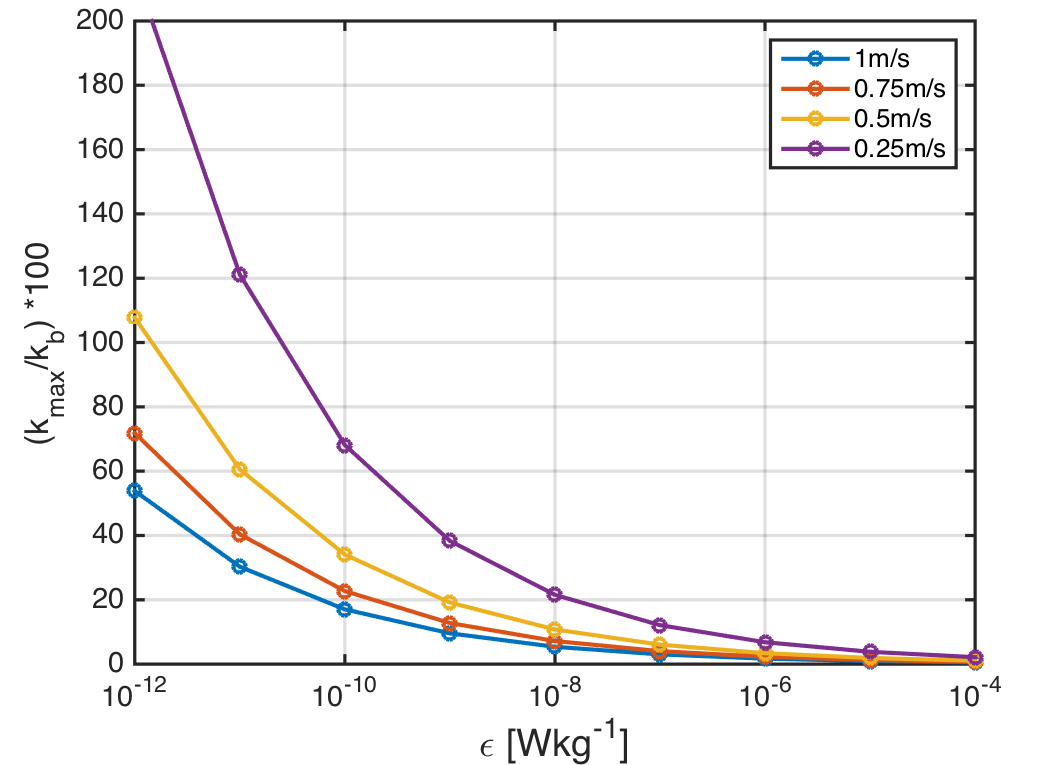
\includegraphics[width=38pc,angle=0]{kbratVsEps.png}\\
  \caption{Ratio of the maximum observed wavenumber $k_{max}=f_{max}/fspd$ to the \DIFdelbeginFL \DIFdelFL{batchelor }\DIFdelendFL \DIFaddbeginFL \DIFaddFL{Batchelor }\DIFaddendFL wavenumber $k_b$ for different values of $\epsilon$, assuming a $f_{max}=15Hz$. Each line is for a different flowspeed.}
  \label{kbratVseps}
\end{figure}

%\begin{figure}[t]
%  \noindent\includegraphics[width=38pc,angle=0]{p_loops2.png}\\
%  \caption{Example of pressure loops during different sea states. *Not sure if we need this.*}
%  \label{}
%\end{figure}


\begin{figure}[t]
  \noindent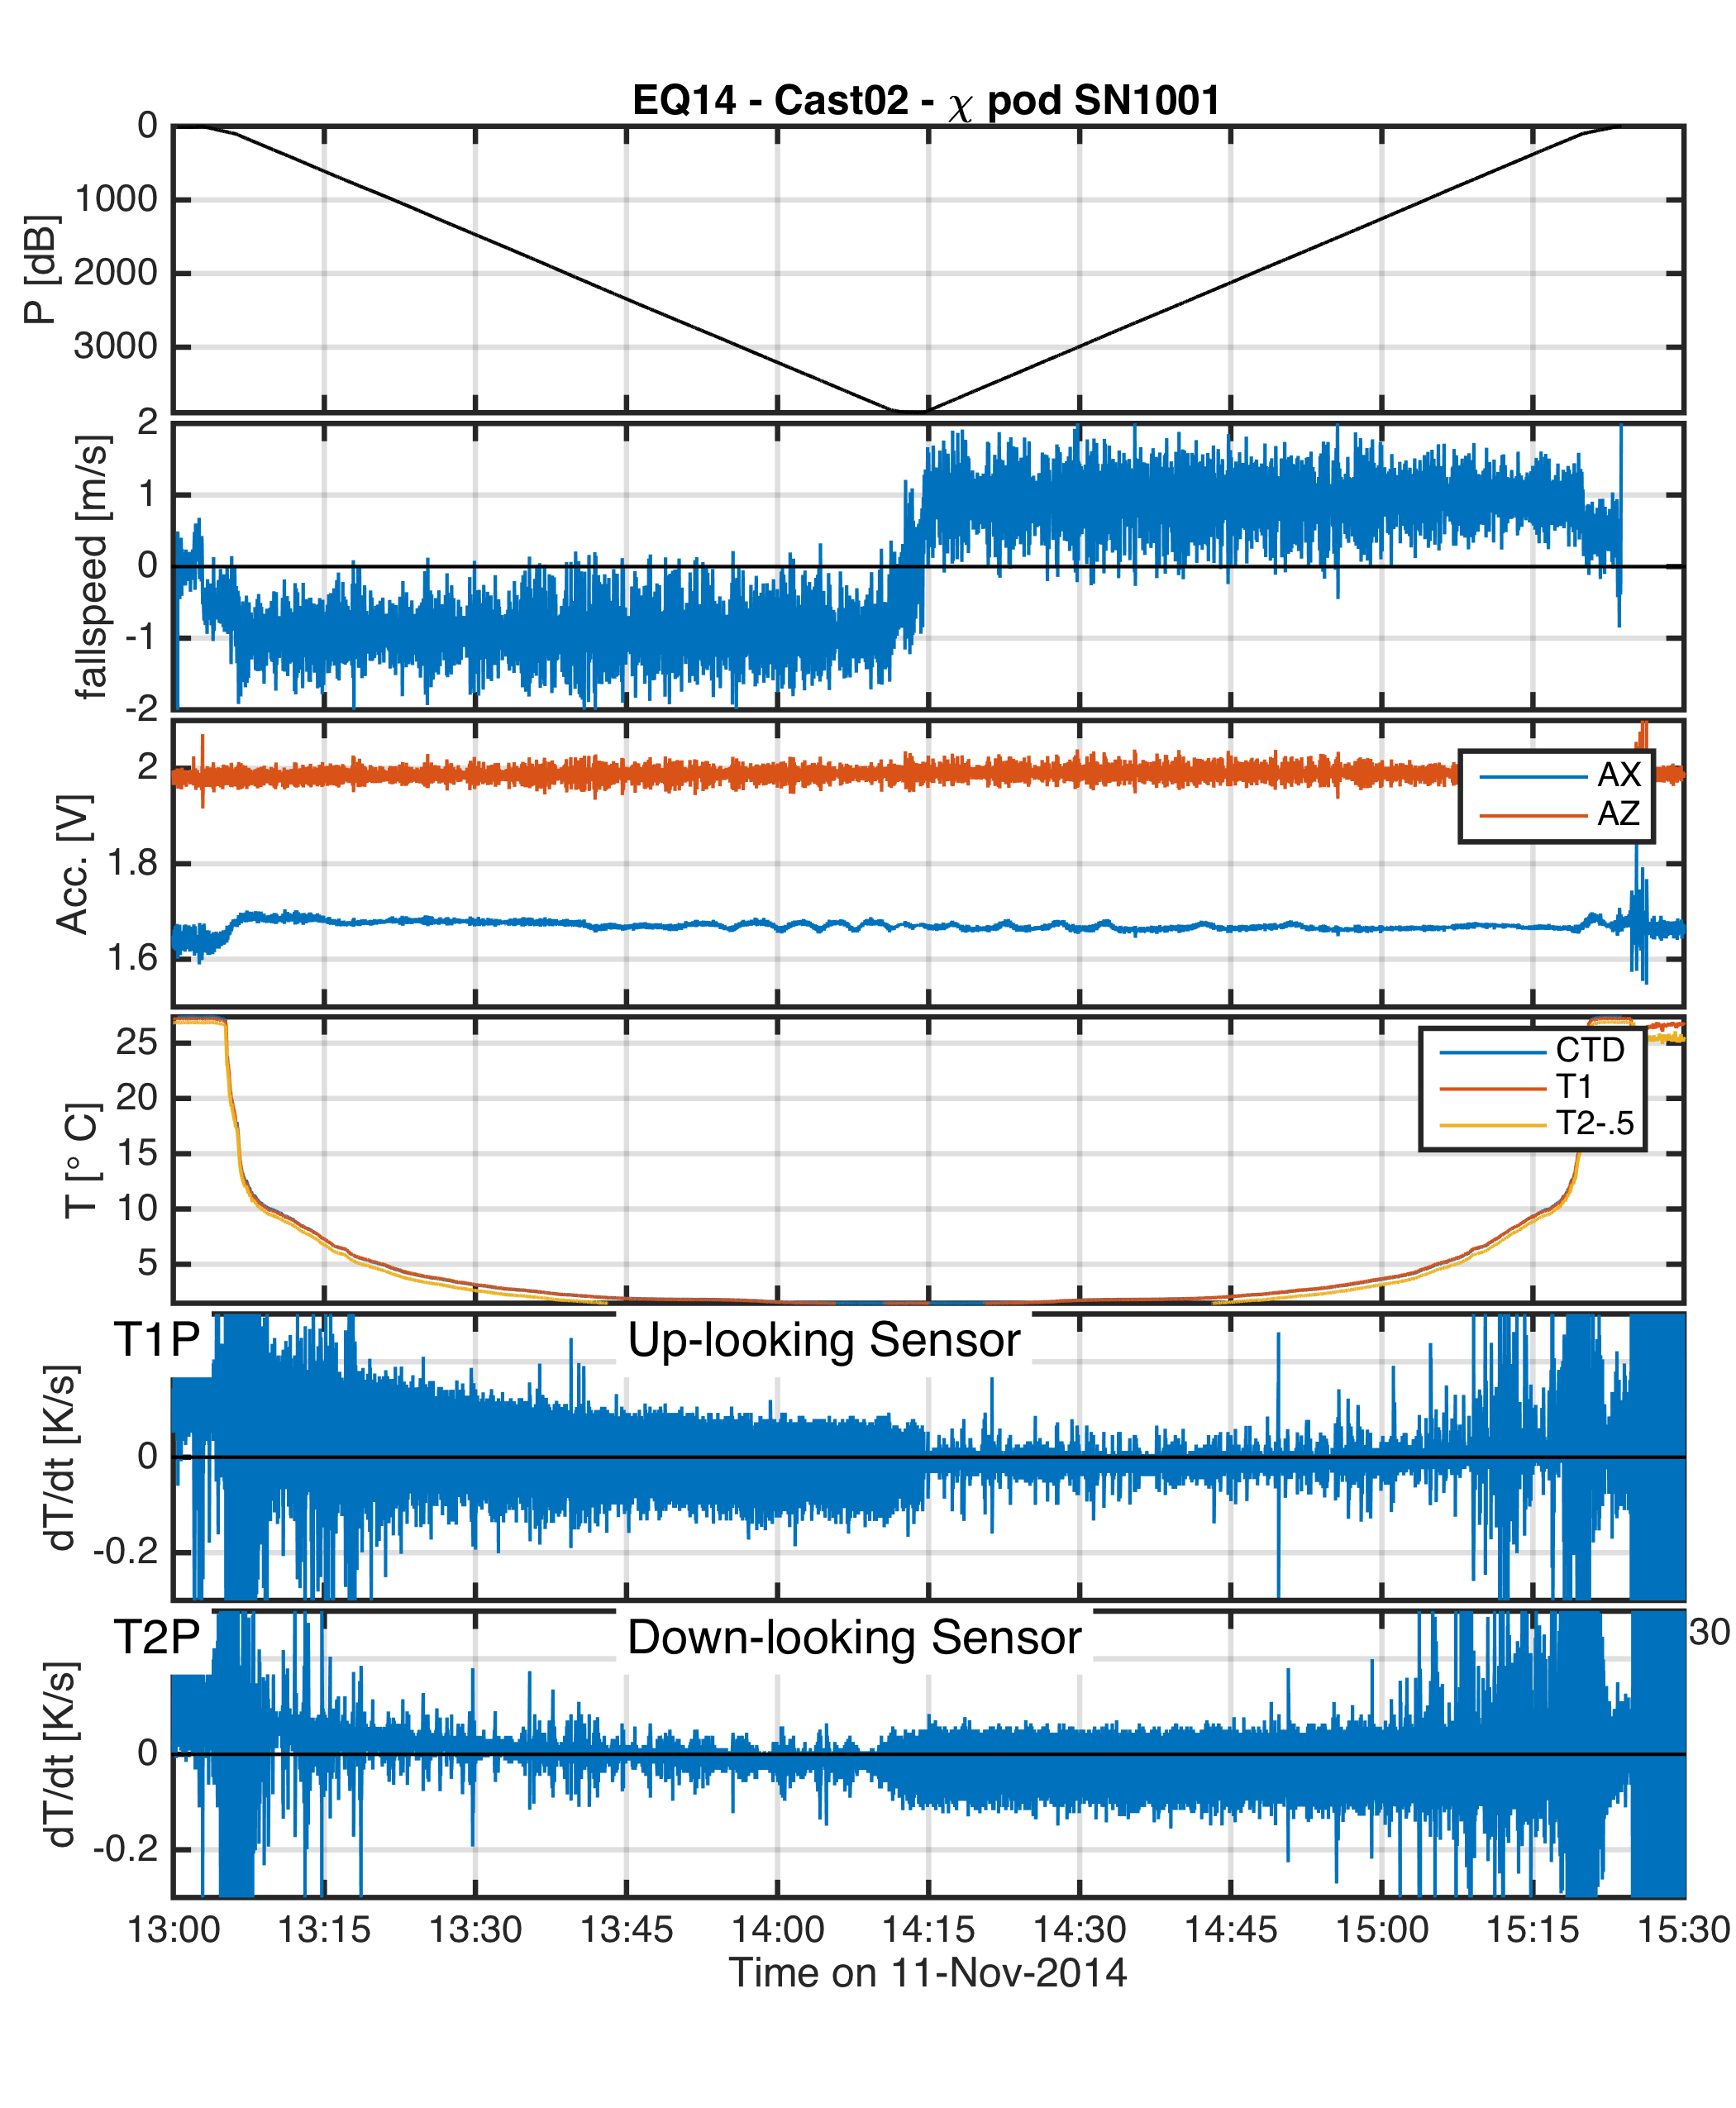
\includegraphics[width=38pc,angle=0]{SN1001_Cast02_Fig5_T_P_dTdz_fspd.png}\\
  \caption{\DIFaddbeginFL {\emJN\DIFaddFL{: add units / calibrate AX/AZ; also check to see if you've plotted dT/dt or -DT/dt.  I think it has the wrong sign/ I think that's what comes out of the electronics; also label T1P and T2P series ``up-looking dT1/dt'' and ``down-looking dT2/dt''}} \DIFaddendFL Example timeseries from one CTD cast during EQ14. a) CTD pressure. b) Fallspeed of CTD ($dp/dt$) .c) Vertical and horizontal accelerations measured by $\chi$-pod. d) Temperature from CTD and (calibrated) $\chi$-pod sensors. T2 is offset slightly for visualization. e) Temperature derivative $dT/dt$ measured by \DIFaddbeginFL \DIFaddFL{the upward-looking }\DIFaddendFL $\chi$-pod sensor T1. f) Temperature derivative $dT/dt$ measured by \DIFaddbeginFL \DIFaddFL{the downward-looking }\DIFaddendFL $\chi$-pod sensor T2. }
  \label{f2}
\end{figure}



\begin{figure}[t]
  \noindent\includegraphics[width=38pc,angle=0]{wind326_specs.png}\\
  \caption{\DIFaddbeginFL {\em \DIFaddFL{JN: why choose an example where epsilon and epsilon chi are so different?  Can we find a better one?}} \DIFaddendFL Example temperature gradient spectra from EQ14. Solid black line show the observed spectra. Dashed magenta line shows the fit theoretical Kraichnan spectra for the $\chi$pod estimates. Purple line is Kraichnan spectra for chameleon $\chi$ and $\epsilon$. Vertical dashed blue lines indicate the minimum and maximum wavenumber used in the $\chi$pod calculation. The \DIFdelbeginFL \DIFdelFL{batchelor }\DIFdelendFL \DIFaddbeginFL \DIFaddFL{Batchelor }\DIFaddendFL wavenumber $k_b$ is also indicated by the cyan line.}
  \label{specexamp}
\end{figure}


% Plot_chiProc_vs_actual_EQ14
\begin{figure}[t]
  \noindent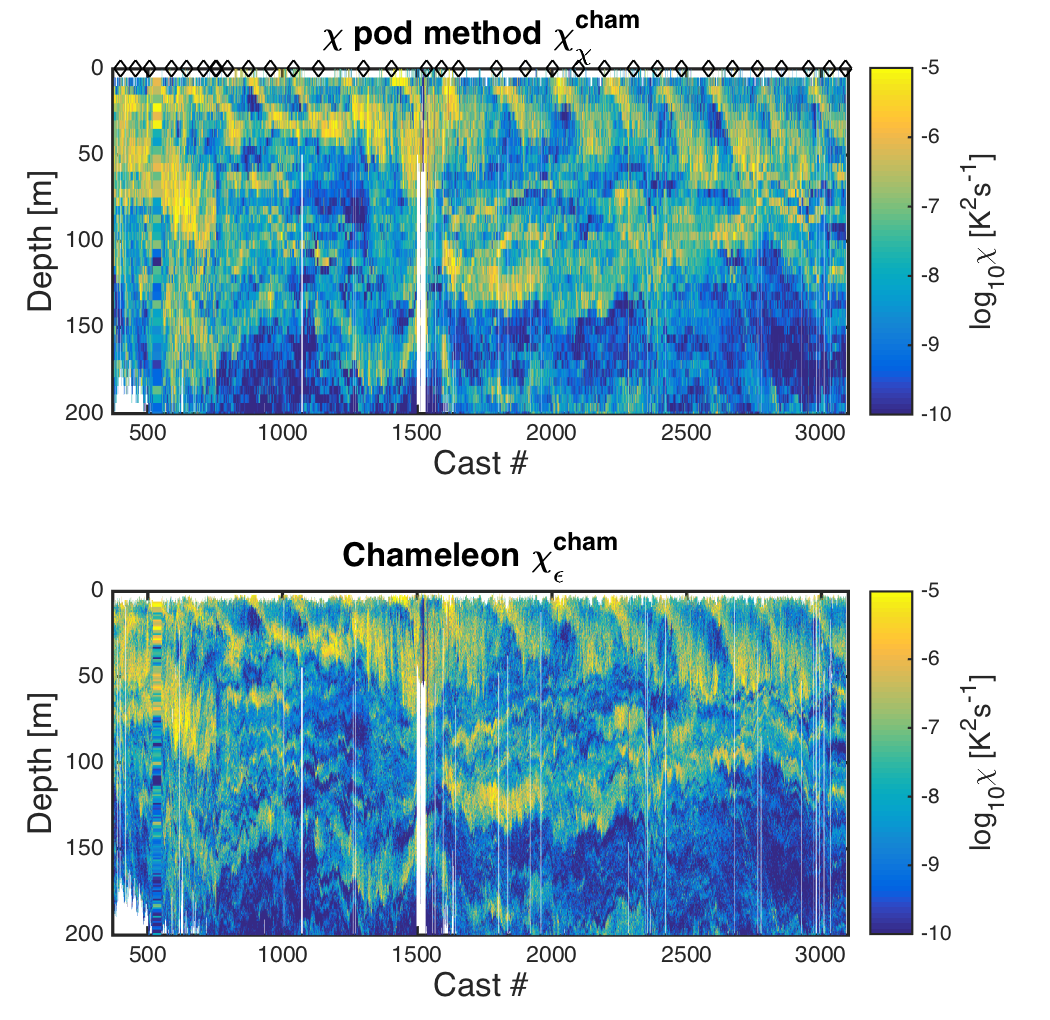
\includegraphics[width=38pc,angle=0]{EQ14_chiVsTrue_chi_zsm10m_fmax7Hz_respcorr0_fc_99hz_gamma20.png}\\
  \caption{Depth-time plots of $log_{10}\chi$ from both methods for EQ14 data. Top: $\chi$pod method. Black diamonds indicate casts used for comparison with CTD-$\chi$pod profiles. Bottom: Chameleon.}
  \label{eq14_eps_pcolor}
\end{figure}


\begin{figure}[t]
  \noindent\includegraphics[width=38pc,angle=0]{EQ14_2dhist_chi_zsm10m_fmax7Hz_respcorr0_fc_99hz_gamma20.png}\\
  \caption{2D histogram of $log_{10}(\chi)$ from chameleon (x-axis) and $\chi$pod method (y-axes). Values from each profile were averaged in the same 5m depth bins. }
  \label{eq14_chi_2dhist}
\end{figure}


% PlotHistKbRatio.m
\begin{figure}[t]
  \noindent\includegraphics[width=38pc,angle=0]{Hist_kbrat.png}\\
  \caption{Histogram of the (left) ratio of the maximum observed wavenumber $k_{max}$ to the \DIFdelbeginFL \DIFdelFL{batchelor }\DIFdelendFL \DIFaddbeginFL \DIFaddFL{Batchelor }\DIFaddendFL wavenumber $k_b$, and (right) fspd for all profiles in EQ14. }
  \label{histkbrat}
\end{figure}

%Scatter_CTDchiVsCham_Pairs.m
\begin{figure}[t]
  \noindent\includegraphics[width=38pc,angle=0]{EQ14_ctdChipod_vs_chamMean_chi_scatter.png}\\
  \caption{Scatter plot of $\chi$ from CTD-$\chi$pod profiles versus the mean of bracketing chameleon profiles. Black dashed line shows 1:1, red are $\pm$ 10 X. **replace with histogram of ratios, or combine into one figure?**}
  \label{eq14_cdtChi_vs_cham}
\end{figure}

%Make_Combined_Cham_for_CTD_pairs.m
% PlotHistChiRatio_CTDchamPairs.m
\begin{figure}[t]
  \noindent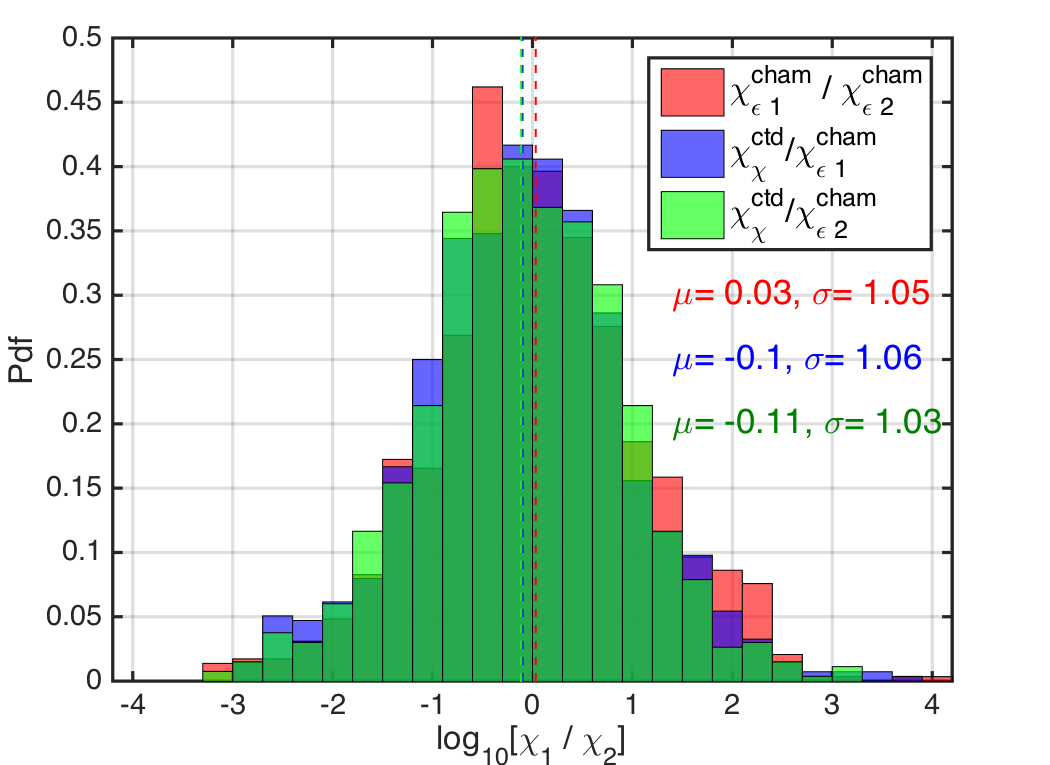
\includegraphics[width=38pc,angle=0]{EQ14_CtdChipod_hist_chi_ratios.png}\\
  \caption{Histogram of $log_{10}$ of the ratio of $\chi$ for nearby casts. The first set is for the before (cham1) and after (cham2) chameleon profiles. the 2nd is CTD-$\chi$pod profiles versus the before(cham1) profiles. The last is CTD-$\chi$pod profiles versus the after(cham2) profiles. Dashed lines show the medians of each set.  Note that bias is small/zero, and the variability (spread) between CTD/cham is similar to the natural variability between cham profiles.}
  \label{eq14_cdtChi_vs_cham_hist}
\end{figure}

% Plot_Pairs_MeanProfile.m
\begin{figure}[t]
  \noindent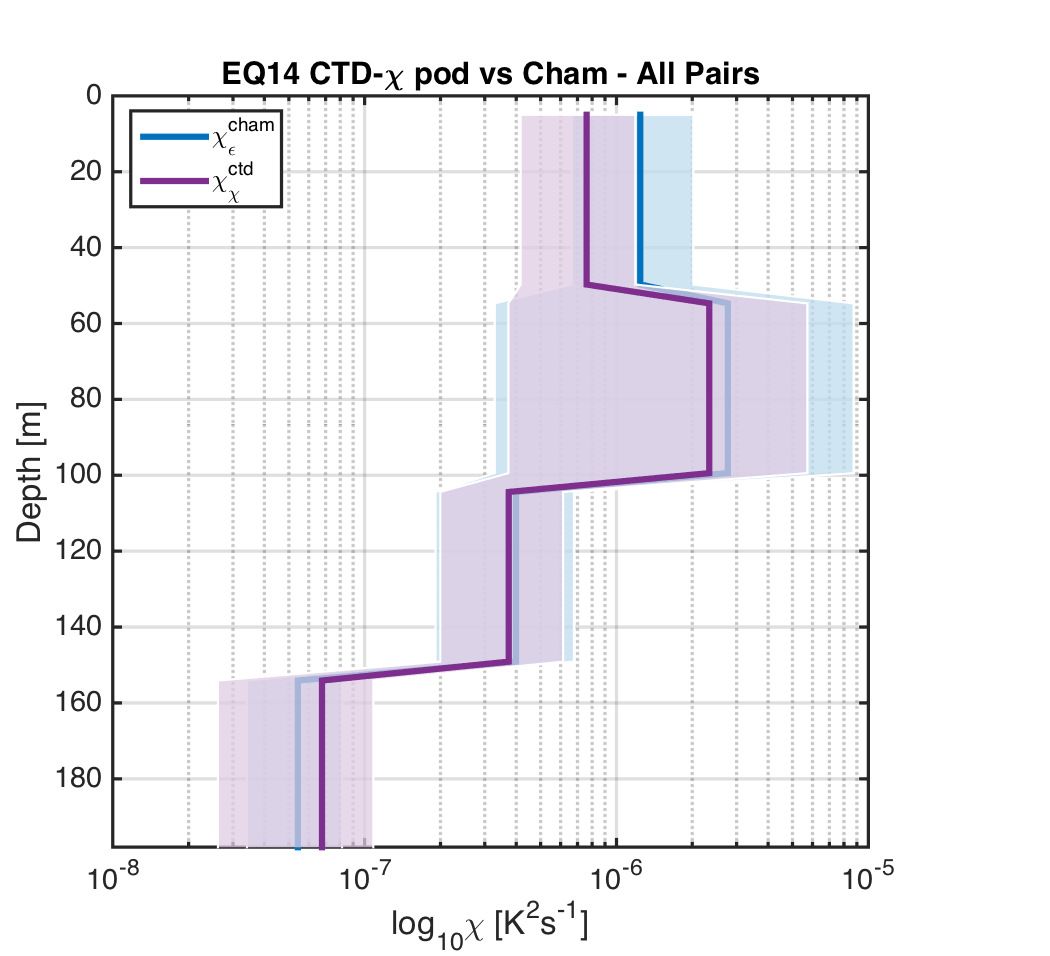
\includegraphics[width=38pc,angle=0]{EQ14_chi_cham_meanProf_all.png}\\
  \caption{Time mean of $\chi$ for all CTD-$\chi$pod - chameleon cast pairs, with 95\% bootstrap confidence intervals.}
  \label{ctd_cham_chi_boot_all}
\end{figure}

% PlotP16chi.m
\begin{figure}[t]
 \noindent\includegraphics[width=38pc,angle=0]{P16N_chi.png}\\
 \caption{Example chipod data from P16N. Top: dTdz. Bottom: $\chi$.}
 \label{p16ex}
\end{figure}

\begin{figure}[t]
  \noindent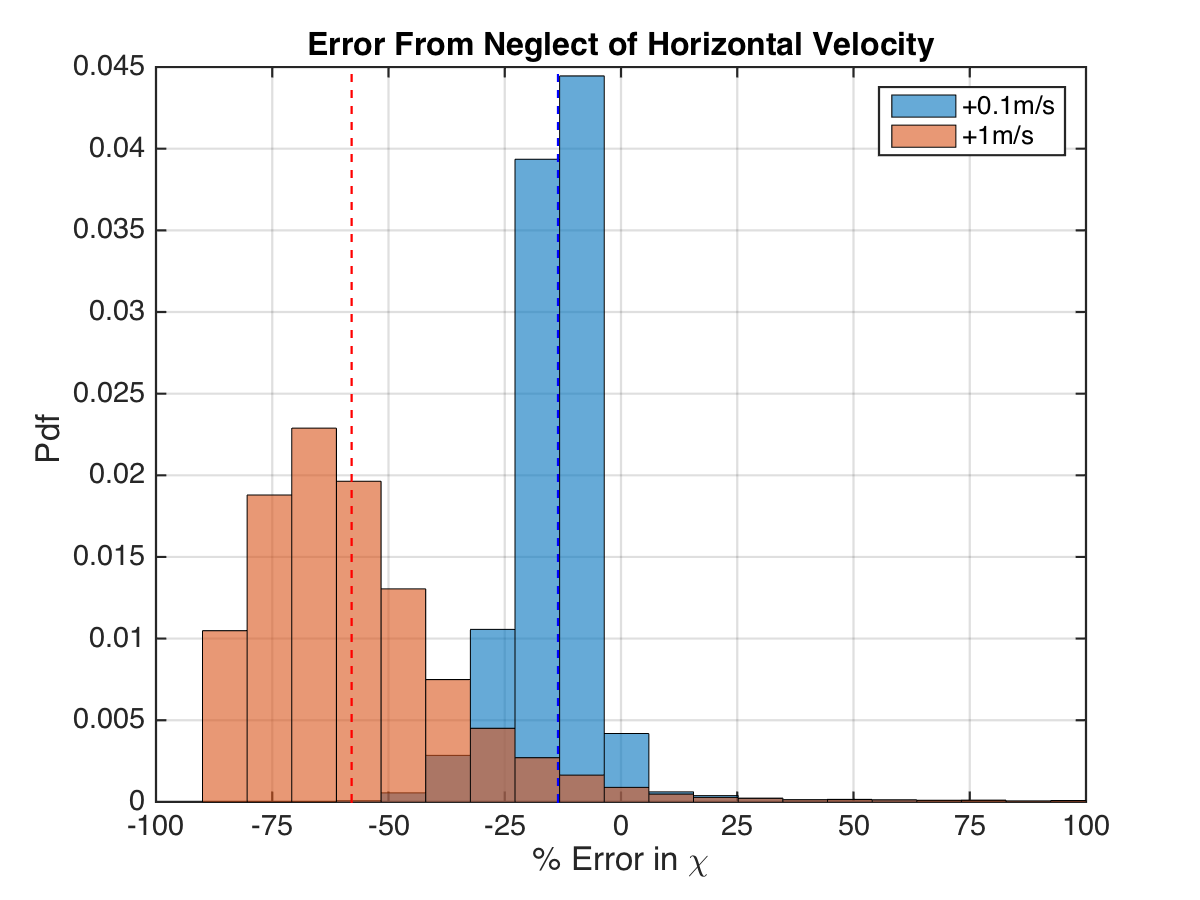
\includegraphics[width=38pc,angle=0]{Hist_perr_fspdvary.png}\\
  \caption{Histogram of \% error for $\chi$ computed with constant added to fallspeed, in order to examine sensitivity to fallspeed.}
  \label{FspdSensHist}
\end{figure}


\begin{figure}[t]
  \noindent\includegraphics[width=38pc,angle=0]{MLEfitsEQ14.png}\\
  \caption{2D histograms of $\chi$ \DIFdelbeginFL \DIFdelFL{from chipod }\DIFdelendFL \DIFaddbeginFL \DIFaddFL{computed using the iterative $\chi$-pod method }\DIFaddendFL (top\DIFaddbeginFL \DIFaddFL{; equation XX}\DIFaddendFL ) and \DIFaddbeginFL \DIFaddFL{the }\DIFaddendFL MLE \DIFaddbeginFL \DIFaddFL{fit }\DIFaddendFL (bottom\DIFaddbeginFL \DIFaddFL{; equation YY}\DIFaddendFL ) \DIFdelbeginFL \DIFdelFL{fits }\DIFdelendFL versus \DIFdelbeginFL \DIFdelFL{chameleon }\DIFdelendFL \DIFaddbeginFL \DIFaddFL{$\chi$ computed from Chameleon }\DIFaddendFL for EQ14 CTD-chipod casts. \DIFaddbeginFL {\em \DIFaddFL{JN - are you really using the CTD chipod casts and not the Chameleon casts?}} \DIFaddendFL Note that the MLE method underestimates $\chi$ at larger magnitudes.}
  \label{mlefits}
\end{figure}



\end{document}